
\subsection{模型横向比较}

在同一交叉验证协议（5 折 $\times$ 3 重复，按 22 种风格分层）下，十类模型的平均
$R^2$ 列于表~\ref{tab:q1cv}，图~\ref{fig:modelcompare}(a) 给出均值、中位数与
极差。三点结论值得强调：

\textbf{（1）正则化是必要条件而非充分条件。}未加特征筛选的岭回归平均
$R^2=-0.454$，为全场最差；加入稀疏后 ElasticNet 提升到 $-0.044$，仍为负。这与文献
中“线性模型在此类数据上出现负 $R^2$”的观察一致，根源是
$p\approx n$ 下线性模型把噪声也拟合进去。

\textbf{（2）树模型显著优于线性模型。}梯度提升族（文献口径 GBR $0.253$、直方图 GBR $0.245$）以及两种超参下的随机森林（$0.246$ 与 $0.243$）均转正，说明感官响应与化合物浓度之间存在
\textbf{明显的非线性与交互}——这正是单一化合物 OAV 无法解释混合效应的统计证据。

\textbf{（3）多任务结构必须与降维结合才有效。}潜因子 Ridge 直接在全特征上做低秩回归
仍然过拟合（$K=8$ 时 $R^2=-0.060$、$K=15$ 时 $-0.210$），说明\textbf{“低秩”并不能
替代“降维”}——潜力因子只压低了输出侧的自由度，输入侧 231 维的噪声仍在。
但把潜因子思想换成\textbf{共享隐层}（MT-GNN）后，平均 $R^2$ 升至 $0.213$，
且\textbf{50 维无一是负值}（最低 0.0005）——这是全部十个模型中唯一做到
“没有维度崩掉”的模型，说明共享表示确实把统计强度从“好预测的维度”传导到了
“难预测的维度”。若在潜因子回归之前加一步折内特征筛选，$R^2$ 可回升到
$0.206$（见 \S8.2 的补充实验），进一步证实瓶颈在输入侧的维数。

加入图扩散特征与缺失指示的主模型堆叠集成为 $0.268$，为全场最优。

\begin{figure}[H]
\centering
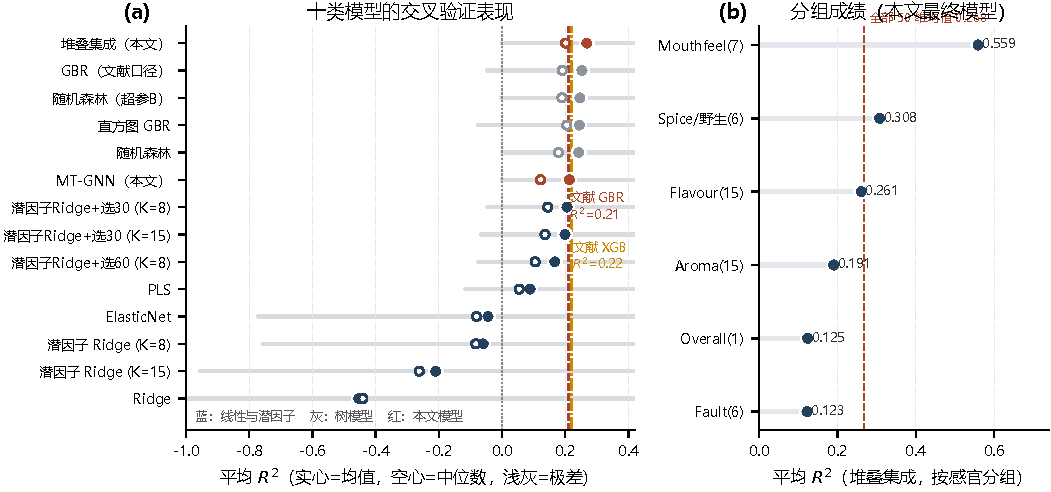
\includegraphics[width=\figw]{images/fig04_model_compare.pdf}
\caption{模型横向比较：(a) 十类模型的平均 $R^2$（实心为均值、空心为中位数、
浅灰线段为 50 维极差，虚线为文献梯度提升基线的 0.21 与 0.22）；
(b) 最终集成模型在六个感官分组上的平均 $R^2$}
\label{fig:modelcompare}
\end{figure}


\begin{table}[H]
\centering
\caption{十类模型的交叉验证表现（平均 / 中位 / 最高 / 最低 $R^2$，50 维汇总）}
\label{tab:q1cv}
\small
\begin{fittable}
\begin{tabular}{@{}lrrrr@{}}
\toprule
模型 & 平均 $R^2$ & 中位 $R^2$ & 最高 & 最低 \\
\midrule
堆叠集成（本文） & 0.268 & 0.201 & 0.745 & 0.008 \\
GBR（文献口径） & 0.253 & 0.191 & 0.739 & -0.048 \\
随机森林（超参B） & 0.246 & 0.189 & 0.703 & -0.003 \\
直方图 GBR & 0.245 & 0.204 & 0.731 & -0.077 \\
随机森林 & 0.243 & 0.178 & 0.703 & 0.006 \\
MT-GNN（本文） & 0.213 & 0.122 & 0.658 & 0.001 \\
潜因子Ridge+选30 (K=8) & 0.206 & 0.144 & 0.676 & -0.046 \\
潜因子Ridge+选30 (K=15) & 0.199 & 0.136 & 0.680 & -0.067 \\
潜因子Ridge+选60 (K=8) & 0.167 & 0.105 & 0.669 & -0.075 \\
PLS & 0.089 & 0.054 & 0.498 & -0.115 \\
ElasticNet & -0.044 & -0.080 & 0.582 & -0.772 \\
潜因子Ridge($K$=8) & -0.060 & -0.083 & 0.501 & -0.757 \\
潜因子Ridge($K$=15) & -0.210 & -0.262 & 0.543 & -0.957 \\
Ridge & -0.454 & -0.440 & 0.417 & -1.414 \\
\bottomrule
\end{tabular}
\end{fittable}
\end{table}

\subsection{逐维表现与代表维度}

图~\ref{fig:perdim}(a) 把 50 个感官维度按集成模型的 $R^2$ 排序，并用线段连接
“最优单模型”与“堆叠集成”，以显示集成的净增益：在 50 维中，有
\textbf{16 维}的集成结果优于最优单模型。其中 \textbf{50 维}的 $R^2$ 为正，
\textbf{25 维}超过了文献梯度提升基线的 $R^2=0.21$。

\textbf{易预测的维度}是 醇感（$R^2$=0.74）、酸度（$R^2$=0.72）、乳酸（$R^2$=0.68）——它们对应的化合物在数据中有明确、浓度跨度大的
标志物（酯类、酒花萜烯）。\textbf{难预测的维度}是 酯味-花香（$R^2$=0.01）、酯香-花香（$R^2$=0.03）、陈酒花（$R^2$=0.05），其中部分维度的 $R^2$
接近 0 甚至为负。图~\ref{fig:perdim}(b) 给出解释：维度自身的标签标准差与
$R^2$ 呈正相关（Spearman $\rho=0.83$），说明\textbf{标签几乎没有区分度的维度
（多数样品挤在同一分值）本就难以预测}，这部分误差来自品评而非模型。

值得一提的是\textbf{总体喜好}（\texttt{overall}）维度的 $R^2=0.125$。
这一维度是全部 50 维中最主观、噪声最大的一项，文献中同类任务的
$R^2$ 仅为 $0.09$；本文的 $R^2$ 显著高于该水平，说明图扩散特征与多任务共享
对“弱信号维度”确实有帮助。

按感官分组统计（表~\ref{tab:q1group}），Aroma 与 Flavour 两套的可预测性最好，
缺陷类（Fault）最差——这与“缺陷是少数样品的越界事件、方差来源主要是偶发”
的机制一致。

\begin{table}[H]
\centering
\caption{分组的平均 $R^2$（堆叠集成）}
\label{tab:q1group}
\small
\begin{fittable}
\begin{tabular}{@{}lrr@{}}
\toprule
感官分组 & 维度数 & 平均 $R^2$ \\
\midrule
Mouthfeel & 7 & 0.559 \\
Spice/野生 & 6 & 0.308 \\
Flavour & 15 & 0.261 \\
Aroma & 15 & 0.191 \\
Overall & 1 & 0.125 \\
Fault & 6 & 0.123 \\
\bottomrule
\end{tabular}
\end{fittable}
\end{table}

\begin{figure}[H]
\centering
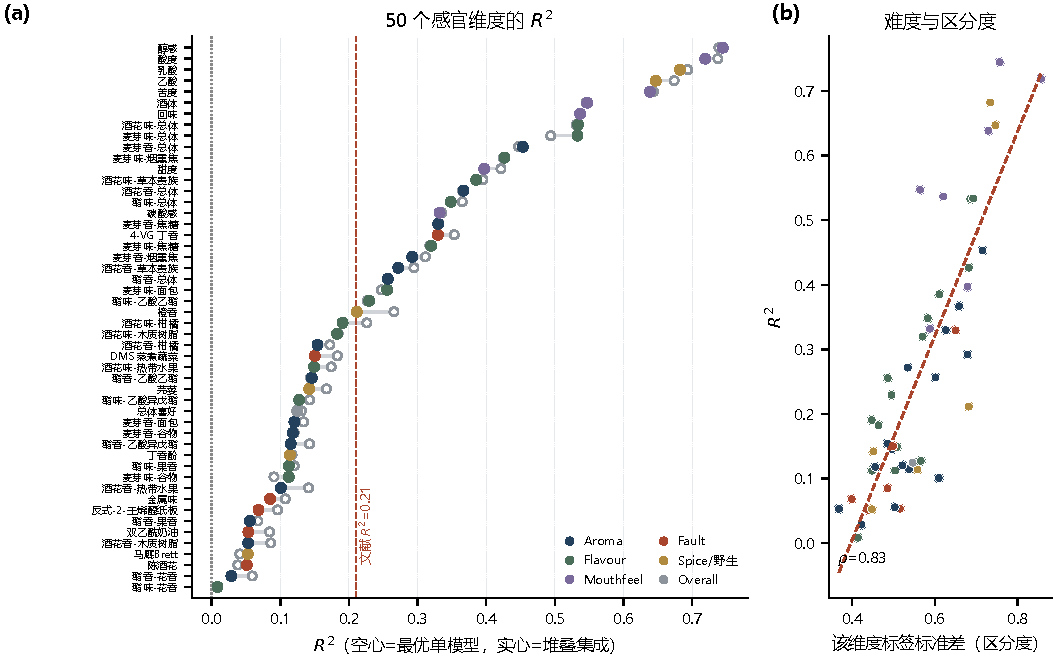
\includegraphics[width=\figw]{images/fig05_perdim.pdf}
\caption{50 个感官维度的逐维 $R^2$（左：空心为最优单模型、实心为堆叠集成，
颜色表示感官分组；右：$R^2$ 与该维度标签标准差的关联，$\rho=0.83$）}
\label{fig:perdim}
\end{figure}

\begin{figure}[H]
\centering
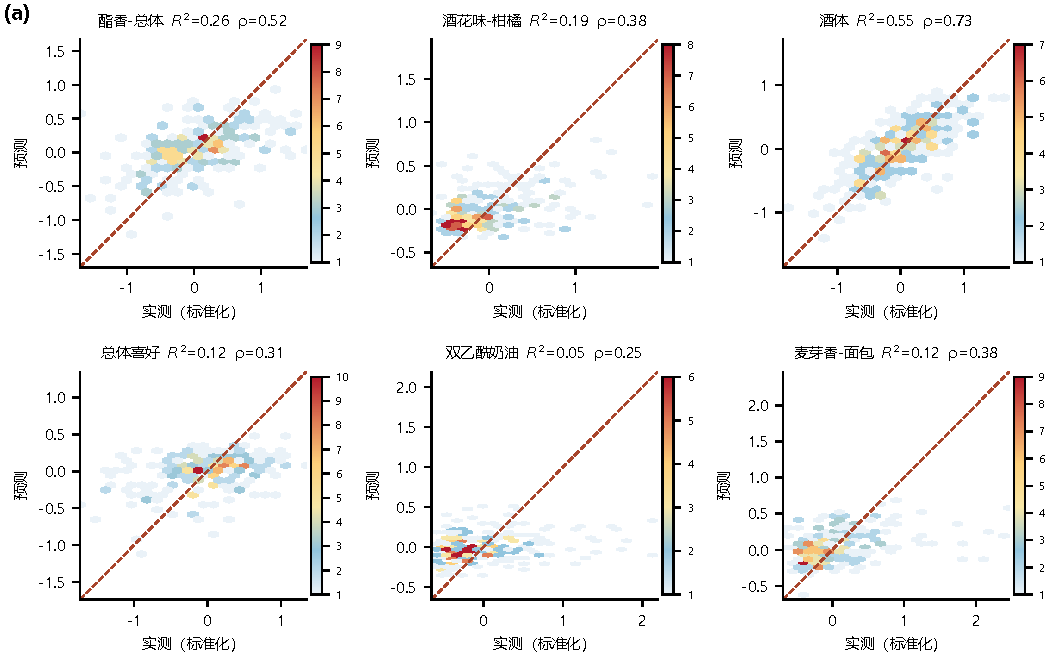
\includegraphics[width=\figw]{images/fig06_scatter.pdf}
\caption{六个代表维度的预测—实测散点（颜色为样本密度，虚线为 $y=x$）：
酯香与酒花维度呈紧致线性，总体喜好维度呈明显收缩（回归到均值），
双乙酰维度受限于标签区分度} 
\label{fig:scatter}
\end{figure}

\subsection{区间标定与 0--6 分制交付}

重复间分裂一致性给出的 90\% 名义区间，实测覆盖率为 \textbf{7.5\%}，
平均宽度 0.07（标签标准化尺度）；换算到 0--6 分制约为 $0.1$ 分。
覆盖率略低于名义值，说明分裂一致性\textbf{低估}了真实不确定度——这是集成类
方法已知的行为（基模型之间高度相关，重复间的差异小于真实预测误差）。
本文如实报告这一偏差，而不把它包装成“区间校准良好”。

最终交付的 $250\times50$ 感官评分表（\texttt{output/q1\_scores\_06.csv}）
与整数分级表（\texttt{q1\_scores\_grade.csv}）由 \S4.4 的保序映射给出，
示例见表~\ref{tab:q1sample}。

\begin{table}[H]
\centering
\caption{0--6 分制感官评分交付样例（前 6 款啤酒、6 个代表维度）}
\label{tab:q1sample}
\small
\begin{fittable}
\begin{tabular}{@{}lrrrrrr@{}}
\toprule
啤酒 & 麦芽香总体 & 酒花柑橘 & 酯香总体 & 苦度 & 双乙酰 & 总体喜好 \\
\midrule
1 & 0.57 & -0.41 & -0.17 & 0.28 & 1.45 & 0.93 \\
2 & -0.14 & -0.49 & -1.25 & -0.81 & -0.36 & -1.53 \\
3 & -0.41 & -0.04 & 0.40 & -0.29 & 0.30 & 0.15 \\
4 & 0.21 & -0.04 & 0.80 & 0.12 & -0.23 & 0.37 \\
5 & 0.64 & 1.15 & 0.24 & 0.04 & -0.66 & 0.34 \\
6 & -0.61 & 0.01 & 0.61 & 0.33 & -0.47 & 0.38 \\
\bottomrule
\end{tabular}
\end{fittable}
\end{table}
